%MIT OpenCourseWare: https://ocw.mit.edu
%RES.18-011 Algebra I Student Notes, Fall 2021
%License: Creative Commons BY-NC-SA 
%For information about citing these materials or our Terms of Use, visit: https://ocw.mit.edu/terms.

\section{One-Parameter Groups, Continued}

\subsection{Review}
Essentially, we want to restrict the image of $\varphi$ to lie in $G$, in order to understand $G$ better.

\begin{qq}
How can we characterize \emph{which} matrices $A$ define one-parameter subgroups satisfying this property?
\end{qq}

As a motivation, the real numbers with addition, $(\RR, +)$, is essentially the simplest one-dimensional group, and here the notion of a one-parameter maps the real numbers into other groups, allowing us to study more complicated groups using the additive structure of the real numbers.

Let's see an example we covered last time.
\begin{example}[Unitary Matrices]
Let $G = U_n \subset GL_n(\CC).$ Last time, we showed that the condition that $e^{tA} \in U_n$ for all $t \in \RR$ is equivalent to requiring that $A^* = -A$\footnote{Note that it is \emph{not} required for $A$ to be in $GL_n$/invertible; it simply has to be some $n \by n$ matrix.}; that is, if and only if $A$ is skew-Hermitian, the one-parameter subgroup described by $A$ maps to only unitary matrices. %check
\end{example}

\subsection{Examples!}

Another example is given by upper triangular matrices.
\begin{example}[Upper Triangular Matrices]% check if done already
Let
\[
G = \left\{ \begin{pmatrix} 1 & \star & \star \\ 0 & 1 & \star \\ 0 & 0 & 1 \end{pmatrix}\right\} \leq GL_3(\RR)
\]
be the real upper triangular matrices. Then the corresponding $A$ for which $e^{tA}  \in G$ for all $t \in \RR$ make up the set of matrices \[\left\{\begin{pmatrix} 0 & \star & \star \\ 0 & 0 & \star \\ 0 & 0 & 0 \end{pmatrix}\right\} \subseteq \text{Mat}_{3 \by 3}(\RR).\]

\end{example}

The one-parameter group is a homomorphism $\varphi(t) = e^{tA},$ for some matrix $A$; in particular, $A$ is $\varphi'(0).$ So finding what $A$ looks like, given $G,$ is done by taking the derivative at $t = 0.$ The image of $\varphi$ lies in $G,$ and since the 1s down the diagonal are not dependent on $t,$ while the upper right entries could be nonzero, 
%If $e^{tA} \in G$ for all $t,$ then taking the derivative at $t = 0$ gives 
\[
A = \frac{d}{dt}\Big|_{t = 0} \begin{pmatrix} 1 & \star & \star \\ 0 & 1 & \star \\ 0 & 0 & 1 \end{pmatrix} = \begin{pmatrix} 0 & \star & \star \\ 0 & 0 & \star \\ 0 & 0 & 0 \end{pmatrix}.
\]

It is also necessary to show the other direction that if $A$ is of such a form, then the associated one-parameter group $\varphi = e^{tA}$ will actually have its image lie in $G.$ If $A \in \left\{\begin{pmatrix} 0 & \star & \star \\ 0 & 0 & \star \\ 0 & 0 & 0 \end{pmatrix}\right\},$ then $A^k = \left\{\begin{pmatrix} 0 & \star & \star \\ 0 & 0 & \star \\ 0 & 0 & 0 \end{pmatrix}\right\}$ for $k \geq 1.$ Then, the exponential is a sum $\sum \frac{1}{k!} A^k,$ so
\[
e^{A} = \begin{pmatrix} 1 & 0 & 0 \\ 0 & 1 & 0 \\ 0 & 0 & 1 \end{pmatrix} + \begin{pmatrix} 0 & \star & \star \\ 0 & 0 & \star \\ 0 & 0 & 0 \end{pmatrix} + \cdots = \begin{pmatrix} 1 & \star & \star \\ 0 & 1 & \star \\ 0 & 0 & 1 \end{pmatrix},
\]
and therefore $e^{tA} \in G.$ So in fact $e^{tA} \in G$ is equivalent to $A$ being upper triangular. 


Now, let's consider the orthogonal matrices.
\begin{example}
Consider the orthogonal matrices $O_n \subset GL_n(\RR).$ For a one-parameter subgroup of $O_n,$ the matrix $A$ must satisfy $(e^{tA})^T = (e^{tA})^{-1}$for all $t.$

This is equivalent to \[e^{tA^T} = e^{-tA}\] for all $t.$\footnote{Writing out the exponential as a sum gives $(e^{tA})^T = e^{t(A^T)}$, and it is clear that the inverse of $e^{tA}$ is $e^{-tA}$.} Taking the derivative $\frac{d}{dt}$, we get $A^Te^{tA^T} = -Ae^{-tA},$ and evaluating at $t = 0$ gives that the possible $A$ are the ones satisfying
\[
\{A^T = -A\}.\footnote{It is also possible to get this simply by the fact that $O_n$ is $U_n \cap GL_n(\RR),$ and so $A$ must satisfy the same property as for the unitary matrices, that $A^* = -A,$ and for real matrices this condition is the same as $A^T = -A.$}\]

Conversely, if $A^T = -A,$ then $e^{tA^T} = e^{-tA},$ which is equivalent to $(e^{tA})^T = (e^{tA})^{-1}$, and so $e^{tA} \in O_n$ when $A^T = -A.$ So these are the correct matrices $A$. 

\end{example}

\subsection{The Special Linear Group \texorpdfstring{$SL_n(\CC)$}{SLn(C)}}

In order to study $SL_n(\CC),$ which is in some sense the first subgroup of matrices that we ever studied, an important identity about the matrix exponential must be established.

\begin{qq}
What about $SL_n(\CC)?$
\end{qq}

\begin{lemma}\label{det trace}
For any $A \in \text{Mat}_{n \by n}(\CC),$ 
\[
\det e^A = e^{\text{trace}(A)}.
\]
\end{lemma}

This property is clearly true for diagonal matrices, and from there we hope that this is true for other matrices as well. For example, for $A = \begin{pmatrix} \lambda_1 & 0 \\ 0 & \lambda_2 \end{pmatrix}, $ 
\[
e^A = \begin{pmatrix}e^{\lambda_1} & 0 \\ 0 & e^{\lambda_2}\end{pmatrix},
\]
and 
\[\det(e^A) = e^{\lambda_1}e^{\lambda_2} = e^{\lambda_1 + \lambda_2} = e^{\text{trace}(A)}.\]

Trying to steamroll through the proof of the lemma becomes very difficult, but fortunately the exponential, determinant, and trace all behave well with respect to conjugation. 

\begin{proof}
We have 
\[
\det(PAP^{-1}) = \det(A), \text{trace}(PAP^{-1}) = \text{trace}(A), e^{PAP^{-1}} = Pe^AP^{-1}.
\]

Thus, if the lemma is true for a matrix conjugate to $A$, it is true for $A$, and so only one representative from each conjugacy class needs to be considered. Then, without loss of generality, we can assume that $A$ is in Jordan canonical form, and the proof follows identically to the diagonal case. We take
$
A = \begin{pmatrix} \lambda_1 & \cdots & \star \\ \vdots & \ddots & \vdots \\ 0 &\cdots  & \lambda_n\end{pmatrix}
$
to be upper triangular and in Jordan form. Then 
$
A^k = \begin{pmatrix} \lambda_1^k & \cdots & \star \\ \vdots & \ddots & \vdots \\ 0 &\cdots  & \lambda_n^k\end{pmatrix},
$
and so
$
e^A = \begin{pmatrix} e^\lambda_1 & \cdots & \star \\ \vdots & \ddots & \vdots \\ 0 &\cdots  & e^\lambda_n\end{pmatrix},
$
so 
\[
\det(e^A) = e^{\sum \lambda_i} = e^{\text{trace}(A)}.
\]
\end{proof}

Now we can take a look at $SL_n(\CC).$

\begin{example}
Consider $A \in \text{Mat}_{n \by n}(\CC)$  such that $e^{tA}  \in SL_n(\CC)$ for all $t \in\RR.$ Then $e^{tA} \in SL_n(\CC),$ and so $\det(e^{tA}) = 1$ for all $t.$ Therefore, by Lemma \ref{det trace}, $e^\text{trace}(tA) = 1$, which is equivalent to stating that $\text{trace}(A) \in 2\pi i \ZZ$ for all $ t \in \RR,$ which is possible only if the trace of $A$ is 0. So the one-parameter groups in $SL_n(\CC)$ are $e^{tA}$ where $A \in \text{Mat}_{n \by n}(\CC)$ is traceless.\footnote{The trace is 0.}
\end{example}

These conditions on $A$ can obviously be combined for different groups $G$. The one-parameter groups in $SU_n$ correspond with the matrices $A$ such that $A^* = -A$ \emph{and} $\text{trace}(A) = 0.$

In particular, the one-parameter groups in $SU_2$ consist of $e^{tA}$ where the $2 \by 2$ matrix $A$ is skew-symmetric and has zero trace.
\begin{example}[$SU_2$]
 For $A = \begin{pmatrix}\alpha & \beta \\ \gamma & \delta \end{pmatrix},$ these conditions end up giving\footnote{Actually going through the process is slightly tedious and not that informative; try it for yourself if you want to!} that
\[
A = \begin{pmatrix} ix_1 & x_2 + ix_3 \\ -x_2 + x_3 & -ix_1\end{pmatrix} = x_1 \begin{pmatrix}i & 0 \\ 0 & -i\end{pmatrix} + x_2 \begin{pmatrix}0& 1 \\ -1 & 0\end{pmatrix} + x_3 \begin{pmatrix}0 & i \\ i & 0\end{pmatrix}.  
\]

These are the matrices that showed up when we studied the equator! We have \[
A = x_1 \mathbb{I} + x_2 \mathbb{J} + x_3 \mathbb{K},
\]
and so $A = c\vec{v}$ for $\vec{v} \in \mathbb{E} \subset SU_2.$\footnote{Because there is no requirement that $\sqrt{x_1^2 + x_2^2 + x_3^2} = 1,$ $A$ does not actually have to be \emph{on} the equator, but it is just some multiple $c$ of a vector $\vec{v}$ on the equator. When $c = 1,$ $A$ is actually on the equator, by the characterization we gave in a previous lecture.} 

Then 
\[
e^{tA} = e^{tc\vec{v}} = \cos(tc)I + \sin(tc)\vec{v}\footnote{This is given by simply writing out the expansion of the matrix exponential as a sum and collecting the terms into a Taylor series for cosine and a Taylor series for sine; since $\vec{v}$ is on the equator, $\vec{v}^2 = -1,$ and so the result is essentially the same as the result that $e^{i\theta} = \cos\theta + i\sin\theta.$} \in \text{Long}_{\vec{v}}\footnote{This is the characterization given in a previous lecture.}.
\]
Essentially, there is a one-parameter subgroup of $SL_n$ for each $\vec{v}$ for some vector $\vec{v}$ on the equator, where the coefficient $c$ in $A = c\vec{v}$ determines the speed at which the subgroup is swept out. The image of $e^{tA}$ simply corresponds to the longitude given by $\vec{v}.$ %, up to the speed that it sweeps it out, correspond to the longitudes. %explain better

\end{example}
%\subsection{idk} %he said something here can you go back and write it down
\subsection{Tangent Vectors} %the bigger picture?

So far, several examples have been shown, but we would like to see what else we can say more generally about one-parameter subgroups. To do so, we will introduce some new tools. %let's see what else we can say about one-parameter subgroups.
\begin{qq}
What else can we say about the sets\footnote{In fact, they will be vector spaces} of matrices $A$ defining one-parameter groups? 
\end{qq}

Since they are given by derivatives at $t = 0,$ corresponding to the identity, the matrices $A$ are "tangent vectors" to $G \leq GL_n(\RR)$ at the identity $I.$ Intuitively, a tangent vector at some point is a vector lying in the tangent plane. %want to look at tangent vectors to $G \leq GL_n(\RR)$ at the identity $I$. 

\begin{center}
    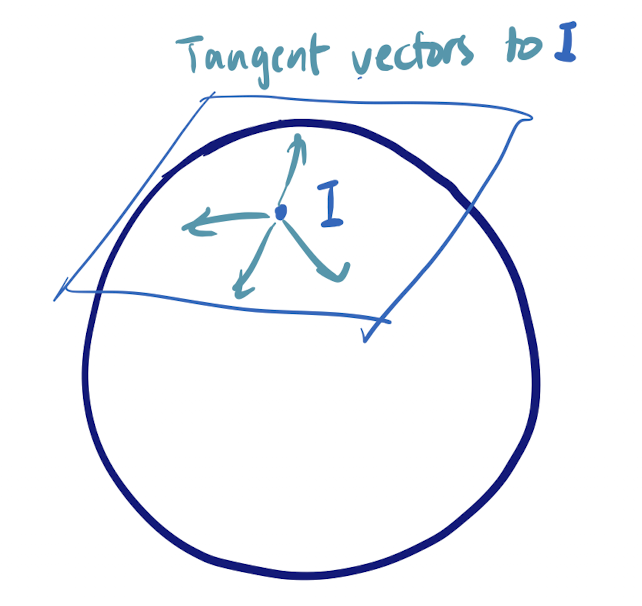
\includegraphics[width=5cm]{Lecture Files and Images/lec32-tangentvector.png}
\end{center}

There are three approaches to rigorously defining tangent vectors. \begin{enumerate}
    \item  The approach taken so far is that a tangent vector will be given by a matrix $A \in \text{Mat}_{n \by n}(\RR)$ such that the corresponding one-parameter group $e^{tA} \in G$ for all $t \in \RR$.\footnote{Every matrix $A$ will define some path in $GL_n;$ if the entire path lives in $G,$ then we can think of $A$ as a tangent vector.}
    \item The second approach is more general, and builds on the idea that a one-parameter group is the trajectory of a particle moving in $G$ in a specific way defined by $\varphi.$ Instead of taking a path that happens to be a homomorphism, take any differentiable path\footnote{Any matrix-valued function} from some interval $f: (-\varepsilon, \varepsilon) \rto GL_n(\RR)$ such that $f(0) = I$ and $f(t) \in (G)$ for all $t.$ Then a tangent vector is simply the velocity at time $t = 0$, $f'(0) \in \text{Mat}_{n \by n}(\RR).$\footnote{The idea is that all the paths through the identity will give velocity vectors (with lots of redundancy), which we will consider as tangent vectors.}
\end{enumerate}

It is not obvious, but it turns out that the first definition is equivalent to the second definition, giving the same subsets of matrices $A$ as tangent vectors. For the first definition, the advantage is that each tangent vector corresponds to only one path through the identity, so there is a bijection. The second approach gives lots of paths through the identity that have a given velocity vector, but it turns out that it is easier to use it to show that the set of tangent vectors actually forms a vector space, called the tangent space.\footnote{There is actually more structure on it, which we will talk about on Friday.}

\begin{enumerate} %START NUMBWRING AT 3
\setcounter{enumi}{2}
    \item Suppose $G$ is defined by polynomial constraints on the matrix entries.\footnote{This approach is not necessary for this class, but it is fun, so we will do it.} For example, the constraints could be that it is upper triangular; then $a_{ij} = 0$ for all $i > j$ is a bunch of polynomial conditions on the matrix entries. Orthogonality can also be phrased as a polynomial condition.
    
    Then, when working with polynomials, the derivative can be mimicked without actually needing to know analysis. We work with an object $\RR[\varepsilon] \coloneqq \RR + \RR \varepsilon$ where $\varepsilon^2 = 0.$\footnote{Here $\varepsilon$ is not some number in $\RR,$ so it is not actually true that $\varepsilon$ must be 0; it is simply a formal construct where we impose the condition that $\varepsilon^2 = 0.$ It is similar to the definition of $i = \sqrt{-1}$; there is no such real number, so we simply define some number satisfying this property. In the same way, we simply define $\RR[\varepsilon]$ to be $\RR + \RR \varepsilon$ for some object $\varepsilon$ satisfying $\varepsilon^2 = 0.$} 
    
    This allows us to define a derivative without actually taking any limits. For example, for $f(x)  = x^2 + 2x,$ evaluating $f$ on $x + \varepsilon \in R[\varepsilon]$ will give
    \begin{align*}
           f(x + \varepsilon) &= (x + \varepsilon)^2 + 2(x + \varepsilon) \\
           &= x^2 + 2x\varepsilon + \varepsilon^2 + 2x + 2\varepsilon\\
           &= x^2 + 2x\varepsilon + 2x + 2\varepsilon\\
           &= (x^2 + 2x) + (2x + 2)\varepsilon.
    \end{align*}
    So with this funky multiplication, any terms of order more than two in $\varepsilon$ disappear, and we get $\frac{f(x + \varepsilon) - f(x)}{\varepsilon} = f'(x),$ even though we haven't actually defined the derivative from an analysis perspective. 
\end{enumerate}

The upshot is that to find $A \in \text{Mat}_{n \by n}(\RR)$, we simply look at $A$ with the property that $I_n + \varepsilon A$, the identity matrix perturbed by $A$, satisfies the same system of equations defining $G$, but in the sense of the funky multiplication of $\RR[\varepsilon]$, where $\varepsilon^2 = 0.$ We'll explain this more on Friday.

\newpage